\chapter{Analisi statica di Data Flow basata su \texttt{CFG}}
Recuperiamo il concetto di analizzatore statico, che è un software che prende
in input un programma, una proprietà $\mathcal{Q}$ e ne restituisce un risultato.

\begin{figure}[H]
    \centering
    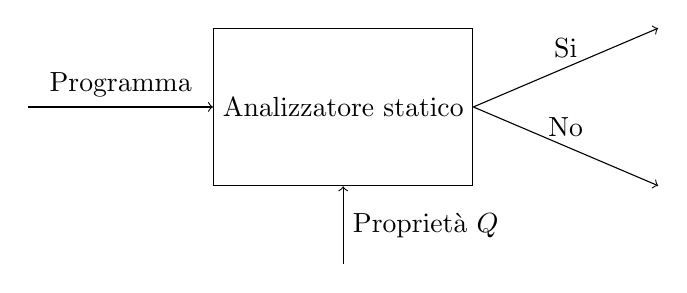
\begin{tikzpicture}
        \node[draw, rectangle, minimum height = 2cm] (b) at (0,6) {Analizzatore statico};
        \draw[->] (-4, 6) -- (b.west) node[midway, above] {Programma};
        \draw[->] (0, 4) -- (b.south) node[midway, right] {Proprietà $Q$};
        \draw[->] (b.east) -- (4, 7) node[midway, above] {Si};
        \draw[->] (b.east) -- (4, 5) node[midway, above] {No};
    \end{tikzpicture}
\end{figure}
L'obiettivo è costruire un analizzatore preciso, ovvero che restituisca sempre
una risposta precisa, ma questa risposta viene data su un'approssimazione della semantica di $\mathcal{P}$.
Su $\mathcal{P}$, in modo decidibile, possiamo dare solamente risposte approssimate.

Attraverso tale analisi ricaviamo informazioni sul punto di programma, spostando l'informazione 
localmente, e andiamo a caratterizzare qual è la collezione di valori raggiunti dal punto di programma. 
L'analizzatore riesce quindi a dare la risposta.

\section{Idea dell'analisi statica}
La semantica del linguaggio di programmazione è una funzione che prende in input un programma scritto in un linguaggio
di programmazione e lo associa in un insieme di denotazioni che descrivono il significato del programma
scritto in $\mathcal{L}$
\[
  \llbracket \cdot \rrbracket : \mathcal{L} \rightarrow \wp(\mathcal{D})
\]
Con $\mathcal{L}$ denotiamo l'insieme dei programmi scritti nel linguaggio $\mathcal{L}$ e con 
$\wp(\mathcal{D})$ denotiamo l'insieme delle sue computazioni, ovvero l'insieme delle tracce di computazione,
ovvero l'insieme di tutte le semantiche dei programmi.

La proprietà in generale, è rappresentata da un sottoinsieme di $\wp(\mathcal{D})$. Ovvero una collezione 
di semantiche che soddisfano la proprietà invariante.
\[
    \mathcal{Q} \subseteq \wp(\mathcal{D})
\]

Dire che $\mathcal{Q} \subseteq \wp(\mathcal{D})$ equivale a dire che $\mathcal{Q}$ è l'insieme di tutti i 
programmi che soddisfano una fissata proprietà, ovvero la proprietà rappresentata.
\section{Analisi statiche}
\begin{itemize}
    \item \textbf{Control Flow Analysis}: si trattano di proprietà analizzabili dalla sintassi del programma,
    su cui non entreremo nel merito.
    \item \textbf{Data Flow Analysis}: guarda come l'informazione fluisce dentro il programma, durante 
    l'esecuzione, quindi riguarda i dati. In tale analisi non si entra nel merito del contenuto dei dati,
    perciò si riesce ad approssimare abbastanza bene sulla sintassi. Non si guarda quindi lo stato della memoria, 
    ma la \textbf{relazione sintattica} tra gli elementi del programma, raggiungendo quindi un accettabile grado 
    di precisione.
    \begin{itemize}
        \item \textbf{Available Expressions}: le classiche analisi ottimizzanti dei compilatori. 
        Riesce a capire se un'espressione è disponibile in un punto di programma, evitando quindi di
        ricalcolarla.
        \item \textbf{Copy Propagation}: permette di capire se delle variabili sono copie di altre 
        variabili, quindi se sono equivalenti.
        \item \textbf{Liveness Analysis}: riguarda le variabili, quindi se una variabile è viva o morta,
        prima di un utilizzo, quindi se è utilizzata in un punto di programma.
        \item \textbf{Reaching Definitions}: definizioni raggiungibili in un punto di programma.
    \end{itemize}
\end{itemize}
Nella definizione intuitiva abbiamo sempre trattato elementi sintattici che raggiungono o hanno 
effetto su un determinato punto di programma. Per questo sono analisi che si approssimano bene sulla 
sintassi.

Le analisi che hanno necessità di entrare nel merito della semantica, che utilizzano altri strumenti 
per analizzare il programma, oltre al \texttt{CFG}, entrando nella memoria per analizzare il dato 
sono le \textbf{analisi distributive}.
\subsection{Analisi statica sul \texttt{CFG}}
Tale analisi si basa su un algoritmo ricorsivo di calcolo della proprietà desiderata sul \texttt{CFG}, visitandolo.

Supponiamo di avere un \texttt{CFG} per ogni procedura, da questa supposizione si ricava che tale analisi può
essere svolta su vari livelli:
\begin{itemize}
    \item \textbf{Locale}: analisi all'interno di un blocco, inteso come collezione massimale di istruzioni senza 
    branching interni, quindi con un'unica entrata e un'unica uscita. 
    \item \textbf{Intra-procedurali}: analisi sui singoli \texttt{CFG} in maniera indipendente.
    \item \textbf{Inter-procedurali}: analisi che considera l'intero programma, si tiene conto anche 
    delle relazioni, ovvero dei ritorni, tra procedure. I \texttt{CFG} non sono 
    isolati ma sono collegati tra loro.
\end{itemize}

Ciò che faremo in relazione alla analisi statica, consiste nel caratterizzare come l'informazione di interesse
viene trasformata dentro il programma. L'arco denota solamente il passaggio di controllo, mentre il nodo 
rappresenta il blocco, dove vi è la modifica dello stato.
Dobbiamo quindi capire come l'informazione di interesse viene trasformata, nella sua versione approssimata.

Questa analisi avviene in due fasi:
\begin{enumerate}
    \item Caratterizzare l'informazione di interesse che entra nel blocco. Combinando le informazioni 
    che arrivano dai blocchi predecessori. Nel caso in cui il blocco abbia più predecessori, l'informazione
    di interesse è la combinazione delle informazioni di interesse che arrivano dai vari predecessori.
    Si parla di combinazione perché dipenderà dal tipo di analisi.
    \item Caratterizzare l'informazione di interesse che esce dal blocco come manipolazione dell'informazione
    in entrata. Il calcolo avviene per punto fisso, partendo da un'ipotetica informazione iniziale tendenzialmente 
    vuota e vengono visitati tutti i nodi del control flow graph, finché l'informazione non si stabilizza, ovvero 
    non viene modificata. A quel punto abbiamo trovato l'invariante dell'informazione di interesse in quel punto di entrata 
    o di uscita del blocco.
\end{enumerate}

\subsubsection{Esempio di ottimizzazioni}
\begin{algorithm}[H]
    \caption{Bubble sort}
    \For{$i \gets n - 2 \textbf{ to } 0$}
    {
        \For{$j \gets 0 \textbf{ to } i$}
        {
            \If{$A[j] > A[j + 1]$}
            {
                $t \gets A[j]$\\
                $A[j] \gets A[j + 1]$\\
                $A[j + 1] \gets t$\\
            }
        }
    }
\end{algorithm}

Il codice intermedio generato è il seguente:


\begin{algorithm}[H]
    \caption{Bubble sort}
        $i \gets n - 2$\\
        $S_5: \textbf{ if } i < 0 \textbf{ goto } S_1$\\
        $j \gets 0$\\
        $S_4: \textbf{ if } j > i \textbf{ goto } S_2$\\
        $t_1 \gets j \cdot 4$\\
        $t_2 \gets \&A$\\
        $t_3 \gets t_2 + t_1$\\
        $t_4 \gets *t_3$\\
        $t_5 \gets j + 1$\\
        $t_6 \gets t_5 \cdot 4$\\
        $t_7 \gets \&A$\\
        $t_8 \gets t_7 + t_6$\\
        $t_9 \gets *t_8$\\
        $\textbf{ if } t_4 \leq t_9 \textbf{ goto } S_3$\\
        $t_{10} \gets j \cdot 4$\\
        $t_{11} \gets \&A$\\
        $t_{12} \gets t_{11} + t_{10}$\\
        $\texttt{temp} \gets *t_{12}$\\
        $t_{13} \gets j + 1$\\
        $t_{14} \gets t_{13} \cdot 4$\\
        $t_{15} \gets \&A$\\
        $t_{16} \gets t_{15} + t_{14}$\\
        $t_{17} \gets *t_{16}$\\
        $t_{18} \gets j \cdot 4$\\
        $t_{19} \gets \&A$\\
        $t_{20} \gets t_{19} + t_{18}$\\
        $*t_{20} \gets t_{17}$\\
        $t_{21} \gets j + 1$\\
        $t_{22} \gets t_{21} \cdot 4$\\
        $t_{23} \gets \&A$\\
        $t_{24} \gets t_{23} + t_{22}$\\
        $*t_{24} \gets \texttt{temp}$\\
        $S_3: j \gets j + 1$\\
        $\textbf{ goto } S_4$\\
        $S_2: i \gets i - 1$\\
        $\textbf{ goto } S_5$\\
        $S_1: \textbf{ return }$\\
\end{algorithm}
In questo caso ci sono diverse espressioni ridondanti, ad esempio $j \cdot 4$ oppure $j + 1$.
Ci chiediamo se è necessario rivalutare tali espressioni oppure possiamo utilizzare il risultato
calcolato precedentemente.

Applicando varie ottimizzazioni, si ottiene il seguente codice:

\begin{algorithm}[H]
    \caption{Bubble sort ottimizzato}   
    $i \gets n - 2$\\
    $t_{27} \gets i \cdot 4$ \\
    $t_{28} \gets \&A$\\
    $t_{29} \gets t_{28} + t_{27}$\\
    $t_{30} \gets *t_{29}$\\
    $S_5: \textbf{ if } i < 0 \textbf{ goto } S_1$\\
    $t_{25} \gets t_{28}$\\
    $t_{26} \gets t_{30}$\\
    $S_5: \textbf{if } t_{25} > t_{29} \textbf{ goto } S_2$\\
    $t_4 \gets *t_{25}$\\
    $t_9 \gets *t_{26}$\\
    $\textbf{if } t_4 \leq t_9 \textbf{ goto } S_3$\\
    $\texttt{temp} = *t_{25}$\\
    $t_{17} \gets *t_{25}$\\
    $*t_{25} \gets t_{17}$\\
    $*t_{26} \gets \texttt{temp}$\\
    $S_3: t_{25} \gets t_{25} + 4$\\
    $t_{26} \gets t_{26} + 4$\\
    $\textbf{goto } S_4$\\
    $S_2: t_{29} \gets t_{29} - 4$\\
    $\textbf{goto } S_5$\\
    $S_1: \textbf{ return }$\\
\end{algorithm}

Il codice risultante è molto più compatto, e più efficiente, in quanto non vengono più eseguite
espressioni ridondanti.
\section{Available Expressions}
Supponiamo di avere a disposizione tale codice intermedio:

\begin{algorithm}[H]
  $z \gets 1$\\
  $y \gets M[5]$\\
  $A: x_1 \gets y + z$\\
  \dots\\
  $B: x_2 \gets y + z$\\
\end{algorithm}
Nei blocchi $A$ e $B$ abbiamo la stessa espressione, la domanda che dovrebbe sorgerci è se è necessario
rivalutare l'espressione $y + z$ nel blocco $B$ oppure possiamo utilizzare il risultato calcolato nel blocco $A$.
Non è però detto che si arrivi al punto $B$ dopo aver eseguito il blocco $A$, o che le variabili 
$y$ e $z$ non siano state modificate nel frattempo.

Non è così banale capire se è necessario o meno rivalutare l'espressione, tipicamente queste analisi 
sono fatte per ottimizzare il codice. Tipicamente nella conversione da codice ad alto livello a codice
intermedio, e può essere che in tali conversioni si generino delle espressioni ridondanti, che possono
eseguire eccessivi accessi alla memoria, quindi si vuole evitare di rivalutare l'espressione.

Le available expressions si pongono il quesito di capire se un'espressione
viene ricalcolata in in modo identico in un altro punto di programma.

Se dimostriamo che l'espressione calcolata al punto $A$ arriva anche al punto $B$, possiamo 
modificare il codice, ma per poterlo fare la risposta deve essere certa, senza alcun margine di errore.
Non dobbiamo quindi classificare come ridondanti espressioni che non lo sono, in quanto potremmo
modificare il codice in modo errato.
È ammesso non catturare tutti i calcoli ridondanti perché alla peggio il calcolo sarà meno efficiente, 
ma non avrò modificato la semantica del programma.
\subsection{Definizione formale di available expressions}
\begin{tcolorbox}[title = Espressione disponibile in una variabile $x$ al punto $p$]
    Un'espressione $e$ è disponibile in una variabile $x$ al punto $p$ se:
    \begin{itemize}
        \item $e$ deve essere stata valutata in un punto $q$ precedente a $p$ e 
        salvata in una variabile $x$.
        \item Sia $x$ che tutte le variabili usate in $e$ non devono essere state modificate
        tra la valutazione di $e$ e il punto $p$.
    \end{itemize}
\end{tcolorbox}
\begin{figure}[H]
    \centering 
    \begin{tikzpicture}
        \node[draw, circle, minimum width = 1.3cm] (s) at (0, 2.5)
        {Start};

        \node[draw, circle, minimum width = 1.3cm] (q) at (0, 0) {$k_i$} node[midway, right = 0.7cm] {$x \gets e$};
        
        \node[draw, circle, minimum width = 1.3cm] (p) at (0, -2.5) {$k_n$};
    
        \draw[->,decorate,decoration={snake,amplitude=.4mm,segment length=2mm,post length=1mm}]
        (q) to node[auto, swap] {} (p);
        \draw[->,decorate,decoration={snake,amplitude=.4mm,segment length=2mm,post length=1mm}]
        (s) to node[auto, swap] {} (q);
        \draw[decorate, decoration={calligraphic brace, amplitude=6pt, mirror, raise=5pt, aspect=0.5}]
        (-1,-0.2) -- (-1, -2.3) node[midway,left = 0.5] {$k_{i+1}$};
    \end{tikzpicture}
\end{figure}

Sia $\pi = k_1, \dots, k_n$ dal punto $v$ al punto $p$. L'espressione è disponibile in $x$ al
punto $p$ se:
\begin{itemize}
    \item $\pi$ che contiene $k_i = x \gets e$.
    \item Nessuno tra gli archi $k_{i + 1}, \dots, k_n$ è etichettato con un 
    assegnamento ad una variabile in $x \cup \texttt{Var}(e)$.
\end{itemize}
\begin{equation}
    \texttt{Avail}(n) =
    \begin{cases}
        \varnothing & \text{se } n_0 = n\\
        \bigcap_{m \in \texttt{Pred}(n)} \texttt{AvailOut}(m)
    \end{cases}
\end{equation}
Ogni cammino che arriva al punto di programma che stiamo analizzando deve avere quella espressione come disponibile.
\begin{figure}[H]
    \centering
    \begin{tikzpicture}
        \node[draw, circle, minimum width = 1.3cm] (n) at (-2, 0) {$n$};
        \node[] (k) at (0, 0) {$\dots$};
        \node[draw, circle, minimum width = 1.3cm] (m) at (2, 0) {$m$};
        \node[draw, circle, minimum width = 1.3cm] (p) at (0, -4) {$p$};
        \node at (0, -3) {$\bigcap$};

        \draw[->] (n) to node[auto, swap] {} (p);
        \draw[->] (m) to node[auto, swap] {} (p);
    \end{tikzpicture}
\end{figure}

Per calcolare ciò che è disponibile in uscita da un blocco, dobbiamo caratterizzare ciò che è disponibile
in uscita calcolando come il blocco manipola l'informazione disponibile in ingresso.
\begin{equation}
    \texttt{AvailOut}(n) = \texttt{Gen}(m) \cup (\texttt{AvailIn}(n) \setminus \texttt{Kill}(m))
\end{equation}
Il blocco può manipolare espressioni e di conseguenza può generare nuove espressioni disponibili 
o può uccidere espressioni disponibili in ingresso.

Vediamo la presenza di \textbf{ricorsione} nella definizione di available expressions, poiché abbiamo 
un \texttt{AvailOut} che dipende da un \texttt{AvailIn} e viceversa, quindi il calcolo di punto fisso.

Associamo ad ogni nodo un'informazione chiamata $\texttt{AvailIn}(n)$ che contiene le espressioni 
disponibili in ingresso al nodo $n$.
Il processo inizia con l'inizializzazione, in questo caso supponiamo che all'inizio il primo 
blocco non abbiamo disponibile nessuna espressione. Gli altri blocchi saranno di conseguenza popolati 
con l'elemento neutro dell'operazione di intersezione, ovvero che tutto sia disponibile.
\begin{equation}
    \texttt{AvailIn}(n) =
    \begin{cases}
        \varnothing & \text{se } n_0 = n\\
        \{x \gets e \mid x:=e \textit{ è nel }\texttt{CFG}\}\\
    \end{cases}
\end{equation}
Combinando tali formule otteniamo la seguente equazione ricorsiva di punto fisso che posso calcolare sul \texttt{CFG}:
\begin{equation}
    \texttt{AvailIn}(n) = \bigcap_{m \in \texttt{Pred}(n)} \texttt{Gen}(m) 
    \cup (\texttt{AvailIn}(n) \setminus \texttt{Kill}(m))
    \label{eq:availableexpressions}
\end{equation}
\subsubsection{Espressione generata}
\begin{equation}
    \texttt{Gen}(n) = \{x \gets e \mid x:=e \in b, x \notin \texttt{Var}(e)\}
\end{equation}
\subsubsection{Espressione uccisa}
\begin{equation}
    \texttt{Kill}(n) = \{x \gets e \mid \exists y := e' \in n , y \in \texttt{Var}(e) \vee x = y\}
\end{equation}
\subsection{Algoritmo di available expressions}
La generazione dell'informazione iniziale altro non è che la costruzione di \texttt{Gen} e \texttt{Kill}
che dipende dalla sintassi del blocco e non dal calcolo.

\begin{algorithm}[H]
    \DontPrintSemicolon
    \SetKwFunction{FInit}{Init}
    \SetKwFunction{FDeexpr}{DEExpr}
    \SetKwFunction{FexprKill}{ExprKill}
    \SetKwProg{Fn}{Function}{:}{}
    \ForEach{block b}{\FInit(b)\;}
    %funzione
    \caption{Generazione dell'informazione iniziale}
    \label{alg:init}

    \Fn{\FInit{$b$}}{
        \FDeexpr(b) $ \gets \varnothing $\;
        \FexprKill(b) $ \gets \varnothing $\;
        \For{$i \gets 1 \textbf{ to } k$}{
            \If{$y \notin \FexprKill(b) \land z \notin \FexprKill(b)$}{
                \textbf{add} $x \gets (y \circ z)$ \textbf{to} \FDeexpr(b)\;
            }
            \textbf{add} $x$ \textbf{to} \FDeexpr(b)\;
        }
        \KwRet\;
    }
\end{algorithm}

Una volta che abbiamo l'informazione iniziale, possiamo calcolare l'available expressions.

\begin{algorithm}[H]
    \DontPrintSemicolon
    \SetKwFunction{FavailableIn}{AvailIn}
    \caption{Available expressions}
    \label{alg:availablealgorithm}
    \For{$i \gets 1 \textbf{ to } N - 1$}{
        AvailIn($i$) $ \gets \{\texttt{AllExpr}\} $\;
        AvailIn(0) $ \gets \varnothing $\;
    }
    changed $ \gets \textbf{true} $\;
    \While{changed}{
        changed $ \gets \textbf{false} $\;
        \For{$i \gets 1 \textbf{ to } N - 1$}{
            old $ \gets $ AvailIn($i$)\;
            AvailIn($i$)\;
            \If{old $\neq$ AvailIn($i$)}{
                changed $ \gets \textbf{true} $\;
            }
        }
    }
\end{algorithm}

\subsection{Esempio}

\begin{minipage}{0.5\textwidth}
    Consideriamo il seguente programma:

    \begin{algorithm}[H]
        $y \gets 1$\;
        \While{$x \geq 1$}{
            $y \gets y \cdot x$\;
            $x \gets x - 1$\;
        }
    \end{algorithm}

    gli assegnamenti sono:
    \begin{itemize}
        \item $y \gets 1$
        \item $y \gets y \cdot x$
        \item $x \gets x - 1$
    \end{itemize}
    Osserviamo che in $y \gets y \cdot x$ abbiamo la variabile modificata
    $y$ anche tra le variabili dell'espressione, perciò non sarà disponibile. 
    Lo stesso varrà per $x \gets x - 1$.

    L'insieme di tutti gli assegnamenti è:
    \[
        \texttt{AllExpr} = \{y \gets 1\}
    \]
    \end{minipage} 
    \begin{minipage}{0.5\textwidth}
    \begin{figure}[H]
        \centering
        \begin{tikzpicture}[node distance={12mm}, main/.style = {draw, rectangle}] 
            \node[main] (1) {1. $y \gets 1$};
            \node[main] (2) [below =of 1] {2. $x \geq 1$};
            \node[main] (5) [below right =of 2] {3. $y \gets x \cdot y$};
            \node[main] (4) [below =of 5] {4. $x \gets x - 1$};
            \node[main] (6) [below left=of 2] {5. \texttt{exit}};
            \draw[->] (1) -- (2);
            \draw[->] (2) -- (5);
            \draw[->] (2) -- (6);
            \draw[->] (5) -- (4);
            \draw[->] (4) -- (2);
        \end{tikzpicture}
    \end{figure}
    \end{minipage}

    Costruiamo per ogni blocco l'insieme di espressioni generate e uccise:
    \begin{itemize}
        \item $b_1$: \texttt{Gen}(1) $= \{y \gets 1\}$, \texttt{Kill}(1) $= \{ y \gets 1 \}$
        \item $b_2$: \texttt{Gen}(2) $= \varnothing$, \texttt{Kill}(2) $= \varnothing$
        \item $b_3$: \texttt{Gen}(3) $= \varnothing$, \texttt{Kill}(3) $= \{ y \gets 1 \}$
        \item $b_4$: \texttt{Gen}(4) $= \varnothing$, \texttt{Kill}(4) $= \varnothing$
    \end{itemize}

    Seguendo la formula per il calcolo dell'available expressions (Eq. \ref{eq:availableexpressions}), e l'algoritmo 
    \ref{alg:availablealgorithm}, otteniamo:
    \begin{figure}[H]
        \centering
        \renewcommand{\arraystretch}{2}
        \begin{tabular}{|>{\centering\arraybackslash}m{5em}|m{5em}|m{5em}|m{5em}|m{5em}|m{5em}|}
            \hline
            & \textbf{1} & \textbf{2} & \textbf{3} & \textbf{4} & \textbf{$\dots$} \\
            \hline
            \textbf{1} & $\varnothing$ & $\varnothing$ & $\varnothing$ & $\varnothing$ & $\dots$ \\
            \hline
            \textbf{2} & $y \gets 1$ & $y \gets 1$ & $\varnothing$ 
            & $\varnothing$ & $\dots$ \\
            \hline
            \textbf{3} & $y \gets 1$ &$y \gets 1$ & $y \gets 1$ & $\varnothing$ & $\dots$ \\
            \hline
            \textbf{4} & $y \gets 1$ & $\varnothing$ & $\varnothing$  & $\varnothing$ & $\dots$ \\
            \hline
            \textbf{5} & $y \gets 1$  & $y \gets 1$ & $y \gets 1$ & $\varnothing$ & $\dots$ \\
            \hline
        \end{tabular}
    \end{figure}
Quindi alla quarta iterazione abbiamo che non ci sono cambiamenti, quindi l'algoritmo termina e troviamo il punto fisso.
\subsection{Analisi del control flow graph}
Riassumendo l'analisi del control flow graph, abbiamo che l'analisi può essere fatta in modi, forward o backward.

\subsubsection{Forward}
L'idea del forward è che l'informazione si propaga dai blocchi iniziali a quelli finali.
\begin{equation}
    \texttt{FAvailIn}(n) = 
        \begin{cases}
            \texttt{InitInf} & n = n_0\\
            \bigoplus_{m \in \texttt{pred}(n)} \texttt{FAvailOut}(m)
        \end{cases}
\end{equation}
\begin{equation}
    \texttt{FAvailOut}(n) = \texttt{Gen}(n) \cup (\texttt{FAvailIn}(n) \setminus \texttt{Kill}(n))
\end{equation}
La combinazione delle due espressioni ci permette di calcolare l'insieme di espressioni disponibili in un blocco.
\begin{equation}
\texttt{FAvailIn}(n) = \bigoplus_{m \in \texttt{pred}(n)} \texttt{Gen}(m) \cup (\texttt{FAvailIn}(m)
\setminus \texttt{Kill}(m))
\end{equation}
La combinazione deriva dal fatto che si può differenziare in unione o intersezione:
\begin{itemize}
\item \textbf{Unione}: se vogliamo che l'analisi sia \textbf{possibile};
\item \textbf{Intersezione}: se vogliamo che l'analisi sia \textbf{definite}.
\end{itemize}

\subsubsection{Backward}
L'idea del backward è che l'analisi parte dal blocco di uscita e risale il grafo di controllo, quindi:
\begin{equation}
    \texttt{BAvailOut}(n) = 
        \begin{cases}
            \texttt{InitInf} & n = n_f\\
            \bigoplus_{m \in \texttt{succ}(n)} \texttt{FAvailIn}(m)
        \end{cases}
\end{equation}
\begin{equation}
    \texttt{BAvailOut}(n) = \texttt{Gen}(n) \cup (\texttt{BAvailOut}(n) \setminus \texttt{Kill}(n))
\end{equation}
La combinazione delle due espressioni ci permette di calcolare l'insieme di espressioni disponibili in un blocco.
\begin{equation}
\texttt{BAout}(n) = \bigoplus_{m \in \texttt{succ}(n)} \texttt{Gen}(m) \cup (\texttt{BAvailIn}(m)
\setminus \texttt{Kill}(m))
\end{equation}
La combinazione deriva dal fatto che si può differenziare in unione o intersezione:
\begin{itemize}
\item \textbf{Unione}: se vogliamo che l'analisi sia \textbf{possibile};
\item \textbf{Intersezione}: se vogliamo che l'analisi sia \textbf{definite}.
\end{itemize}
\section{Framework per l'analisi}
Formalizziamo il problema dell'analisi statica attraverso la semantica. L'idea è quella di 
riscrivere in funzione della semantica fornire un algoritmo di risoluzione del problema. Ciò 
permette di avere un algoritmo generico che può essere applicato a diversi problemi. La semantica è quindi 
un parametro di tale algoritmo, rendendo la struttura di analisi più modulare.

Il Framework ci permette inoltre di spostare l'attenzione dalle analisi di dataflow, molto più vicine 
alla sintassi, poiché verificano il modo in cui fluiscono i dati, in semantiche che guardano 
la semantica del programma, ovvero il significato del programma.

I passi per la costruzione del framework sono:
\begin{enumerate}
    \item Formalizzare l'informazione astratta che vogliamo osservare;
    \item Definizione l'\textit{abstract edge effect}, ovvero l'effetto che un arco ha sull'informazione astratta 
    (\textit{transfer function});
\end{enumerate}
Una volta definite queste due componenti, costruiamo un sistema di disequazioni (\textit{una 
disequazione per ogni punto di programma}), cercando la miglior soluzione possibile. La 
ricerca della miglior soluzione possibile può seguire due approcci:
\begin{itemize}
    \item \textbf{Naive}: baso la soluzione sullo step precedente.
    \item \textbf{Round Robin}: baso la soluzione sugli step precedenti e sul calcolo attuato nello step attuale,
    per accelerare il processo di convergenza.
\end{itemize}
La soluzione  verrà utilizzata per ottenere la soluzione del sistema che approssima
la soluzione \textbf{MOP} (\textit{Merge 
Over all Paths}).

L'obiettivo è la soluzione più precisa possibile, quindi la soluzione \textbf{MOP}. Tuttavia, quello che possiamo 
calcolare è la soluzione \textbf{MFP} (\textit{soluzione del sistema di disequazioni}). Quando le due soluzioni 
coincidono avremo che la soluzione è la più precisa possibile, se non coincidono nel processo di calcolo è 
stata aggiunta ulteriore perdita di informazione.

\subsection{Framework sull'available expression}
Caratterizziamo l'informazione astratta che vogliamo osservare, ovvero l'insieme di espressioni disponibili 
in un punto di programma. Per rappresentare tale espressione utilizziamo gli insegnamenti $x \gets e$, dove 
$x \notin \texttt{Var}$ e $e \in \texttt{Exp}$. Tale insieme è denominato \texttt{Assign}, a questo punto il dominio 
astratto sarà $\wp(\texttt{Assign}), A \subseteq \texttt{Assign}$.

Caratterizziamo quindi la funzione di trasferimento $\llbracket \cdot \rrbracket^\#\mathcal{A}$. 
Tale funzione è definita sulla semantica astratta, 
per induzione strutturale del \texttt{CFG}.
\[
  k = (u\, \texttt{lab}\, v)  \qquad \cdot \stackrel{\texttt{lab}}{\longrightarrow} \cdot \qquad
  \text{ ovvero }\llbracket \texttt{lab} \rrbracket \mathcal{A}
\]
\begin{itemize}
    \item $\llbracket\texttt{;} \rrbracket^\# \mathcal{A} = \mathcal{A}$
    \item $\llbracket \texttt{NonZero}(e) \rrbracket^\# \mathcal{A} = 
    \llbracket \texttt{Zero}(e) \rrbracket^\# \mathcal{A}
    = \mathcal{A}$
    \item $\llbracket x \gets e \rrbracket^\# \mathcal{A} = 
    \begin{cases}
        \mathcal{A} \setminus \texttt{Occ}(x) & x \in \texttt{Var}(e)\\
        (\mathcal{A} \setminus \texttt{Occ}(x)) \cup \{x \gets e\} & x \notin \texttt{Var}(e)\\
    \end{cases}$
    \\
    dove $\texttt{Occ}(x) = \{x \gets e \in \mathcal{A} \mid y = x \lor x \in \texttt{Var}(e)\}$, ovvero qualunque
    assegnamento dove compare $x$, o a destra o a sinistra del simbolo di assegnamento.
    \item $\llbracket k_0,K_1,\dots,k_n \rrbracket^\# \mathcal{A} = 
    \llbracket k_0 \rrbracket^\# \circ \llbracket k_1 \rrbracket^\# \circ \dots \circ \llbracket k_n \rrbracket^\# \mathcal{A}$
\end{itemize}

\subsection{Espressione definitivamente disponibile}
Un assegnamento $x \gets e$ è definitivamente disponibile in un punto di programma $v$ se è 
disponibile in tutti i cammini che partono dall'\textit{entry point} e arrivano in $v$. Siccome
la soluzione cercata è definitiva, l'operatore di combinazione è l'intersezione.
\begin{equation}
    \mathcal{A}^*[v] = \bigcap \{ \llbracket \pi \rrbracket^\# \varnothing \mid 
    \pi : \texttt{start} \longrightarrow^* v \} 
\end{equation}
Dove $\pi$ rappresenta tutti i cammini. La terminazione di tale calcolo è garantita dal fatto che 
la funzione di trasferimento è monotona e che $\wp(\texttt{Assign})$ non ha catene ascendenti infinite.
In questo particolare caso $\wp(\texttt{Assign})$ è finito, quindi il calcolo termina. Spesso nella 
dataflow analysis si lavora con domini finiti, quindi automaticamente non si hanno catene ascendenti infinite e 
il fatto che sia monotona è garantito dalla definizione della semantica di riferimento.

La perdita di informazione è data dal fatto che consideriamo cammini non eseguibili, dovuto al fatto che 
utilizziamo il \texttt{CFG}. Prendiamo quindi tutti i cammini che contengono i cammini eseguibili.
In generale i cammini eseguibile sono un sottoinsieme stretto dei cammini del \texttt{CFG}, l'identificazione 
dei cammini eseguibili è un problema non decidibile, mentre l'identificazione dei cammini del \texttt{CFG} è un problema
decidibile.

L'altra perdita d'informazione è data dal fatto che non consideriamo il valore delle variabili, potremmo
considerare variabili modificate quando in realtà non lo sono.
\subsection{Computazione della soluzione}
La soluzione è data dalla soluzione del sistema di disequazioni.
Prima di tutto consideriamo ciò che è disponibile al nodo iniziale:
\[
\mathcal{A}[\texttt{start}] \subseteq \varnothing
\] 
In generale utilizziamo contenimento invece di uguaglianza, in quanto si tratta di disequazioni. Costruiamo
disequazioni in modo che la combinazione di ciò che arriva allo stesso nodo avviene per intersezione, sovrastimando ciò 
che avviene nel nodo. 
\[
\mathcal{A}[v] \subseteq \llbracket lab \rrbracket^\# (\mathcal{A}[u]) \qquad \forall k = (u,lab,v)
\]
Quindi l'informazione si propaga attraverso ciò che viene manipolato dall'etichetta, ovvero dall'operazione che su quell'arco viene 
eseguita.

Consideriamo $\mathcal{D} = \wp(\{a,b,c\})$
\begin{itemize}
    \item $x_1 \subseteq \{ a \} \cup x_3$
    \item $x_2 \subseteq x_3 \cap \{a, b \}$
    \item $x_3 \subseteq x_1 \cup \{ c\}$
\end{itemize}
\begin{figure}[H]
    \centering
    \renewcommand{\arraystretch}{2}
    \begin{tabular}{|>{\centering\arraybackslash}m{5em}|m{5em}|m{5em}|m{5em}|m{5em}|m{5em}|}
        \hline
        & \textbf{0} & \textbf{1} & \textbf{2} & \textbf{3} & \textbf{$\dots$} \\
        \hline
        $x_1$ & $\varnothing$ & $\{a\}$ & $\{a, c\}$ & $\{a, c\}$ & $\dots$ \\
        \hline
        $x_2$ & $\varnothing$ & $\varnothing$ & $\{a\}$ 
        & $\{a\}$ & $\dots$ \\
        \hline
        $x_3$ & $\varnothing$ &$\{c\}$ & $\{a, c\}$ & $\{a, c\}$ & $\dots$ \\
        \hline
    \end{tabular}
\end{figure}
Il fix point viene trovato al punto $3$, poiché i valori non cambiano più.

Quando calcoliamo tale soluzione come migliore soluzione del sistema di disequazioni in realtà stiamo
calcolando la soluzione del corrispondente sistema di equazioni.
\begin{tcolorbox}
    Se $f$ è monotona su un reticolo completo, allora il sistema ha miglior soluzione e questa soluzione 
    coincide con la soluzione del sistema di disequazioni.
\end{tcolorbox}
\subsection{Calcolo della soluzione sul fattoriale}
Prendiamo in considerazione la funzione fattoriale.
\begin{figure}[H]
    \centering
    \begin{tikzpicture}[node distance={22mm}, minimum width = 1cm, main/.style = {draw, circle}] 
        \node[main] (1) {1};
        \node[main] (2) [below =of 1] {2};
        \node[main] (5) [below right =of 2] {3};
        \node[main] (4) [below =of 5] {4};
        \node[main] (6) [below left=of 2] {5};
        \draw[->] (1) -- node[left] {$y \gets 1$} (2) ;
        \draw[->] (2) -- node[right] {$\texttt{NonZero}(x > 1)$} (5);
        \draw[->] (2) --  (6) node[above = 1cm] {$\texttt{Zero}(x > 1)$};
        \draw[->] (5) -- node[right] {$y \gets x \cdot y$} (4);
        \draw[->] (4) -- node[left] {$y \gets x -1$} (2);
    \end{tikzpicture}
\end{figure}
Procediamo con l'algoritmo:
\begin{itemize}
    \item $\mathcal{A}[1] \subseteq \varnothing$
    \item $\mathcal{A}[2] \subseteq \llbracket y \gets 1\rrbracket^\#\mathcal{A}[1] = \llbracket y \gets 1\rrbracket^\# \cap 
    \varnothing = \llbracket y \gets 1\rrbracket^\#$
    \item $\mathcal{A}[2] \subseteq \llbracket x \gets x - 1\rrbracket^\#\mathcal{A}[4]$
    \item $\mathcal{A}[3] \subseteq \llbracket \texttt{NonZero}(x > 1)\rrbracket^\#\mathcal{A}[2]$
    \item $\mathcal{A}[4] \subseteq \llbracket y \gets x \cdot y\rrbracket^\#\mathcal{A}[3]$
    \item $\mathcal{A}[5] \subseteq \llbracket y \gets x - 1\rrbracket^\#\mathcal{A}[4]$
\end{itemize}
ovvero
\begin{itemize}
    \item $\mathcal{A}[1] \subseteq \varnothing$
    \item $\mathcal{A}[2] \subseteq \{y \gets 1\} \cap \llbracket y \gets x - 1\rrbracket^\#\mathcal{A}[4]$
    \item $\mathcal{A}[3] \subseteq \llbracket \texttt{NonZero}(x > 1)\rrbracket^\#\mathcal{A}[2]$
    \item $\mathcal{A}[4] \subseteq \llbracket y \gets x \cdot y\rrbracket^\#\mathcal{A}[3]$
    \item $\mathcal{A}[5] \subseteq \llbracket y \gets x - 1\rrbracket^\#\mathcal{A}[4]$
\end{itemize}

Risolviamo quindi il sistema di equazioni:
\begin{itemize}
    \item $\mathcal{A}[1] = \varnothing$
    \item $\mathcal{A}[2] = \{y \gets 1\} \cap (\mathcal{A}[4] \setminus \texttt{Occ}(x))$
    \item $\mathcal{A}[3] = \{y \gets 1\} \cap (\mathcal{A}[4] \setminus \texttt{Occ}(x))$
    \item $\mathcal{A}[4] = \mathcal{A}[3] \setminus \texttt{Occ}(y)$
    \item $\mathcal{A}[5] = \mathcal{A}[2]$
\end{itemize}
\begin{figure}[H]
    \centering
    \renewcommand{\arraystretch}{2}
    \begin{tabular}{|>{\centering\arraybackslash}m{5em}|m{5em}|m{5em}|m{5em}|m{5em}|m{5em}|}
        \hline
        & \textbf{0} & \textbf{1} & \textbf{2} & \textbf{3} & \textbf{$\dots$} \\
        \hline
        $\mathcal{A}[1]$ & $\varnothing$ & $\varnothing$ & $\varnothing$ & $\varnothing$ & $\dots$ \\
        \hline
        $\mathcal{A}[2]$ & $y \gets 1$ & $y \gets 1$ & $\varnothing$ 
        & $\varnothing$ & $\dots$ \\
        \hline
        $\mathcal{A}[3]$ & $y \gets 1$ & $y \gets 1$ & $y \gets 1$ & $\varnothing$ & $\dots$ \\
        \hline
        $\mathcal{A}[4]$ & $y \gets 1$ &$\varnothing$ & $\varnothing$ & $\varnothing$ & $\dots$ \\
        \hline
        $\mathcal{A}[5]$ & $y \gets 1$ &$y \gets 1$ & $y \gets 1$ & $\varnothing$ & $\dots$ \\
        \hline
    \end{tabular}
\end{figure}
Troviamo il punto fisso al punto $3$.

Potremmo accelerare la convergenza dell'algoritmo utilizzando l'algoritmo di \textbf{Round Robin}.
\begin{figure}[H]
    \centering
    \renewcommand{\arraystretch}{2}
    \begin{tabular}{|>{\centering\arraybackslash}m{5em}|m{5em}|m{5em}|m{5em}|m{5em}|m{5em}|}
        \hline
        & \textbf{0} & \textbf{1} & \textbf{2} & \textbf{3} & \textbf{$\dots$} \\
        \hline
        $\mathcal{A}[1]$ & $\varnothing$ & $\varnothing$ & $\varnothing$ & $\varnothing$ & $\dots$ \\
        \hline
        $\mathcal{A}[2]$ & $y \gets 1$ & $y \gets 1$ & $\varnothing$ 
        & $\varnothing$ & $\dots$ \\
        \hline
        $\mathcal{A}[3]$ & $y \gets 1$ & $y \gets 1$ & $\varnothing$ & $\varnothing$ & $\dots$ \\
        \hline
        $\mathcal{A}[4]$ & $y \gets 1$ &$\varnothing$ & $\varnothing$ & $\varnothing$ & $\dots$ \\
        \hline
        $\mathcal{A}[5]$ & $y \gets 1$ &$y \gets 1$ & $\varnothing$ & $\varnothing$ & $\dots$ \\
        \hline
    \end{tabular}
\end{figure}
Raggiungiamo il punto fisso al punto $2$.